%% LyX 2.3.1-1 created this file.  For more info, see http://www.lyx.org/.
%% Do not edit unless you really know what you are doing.
\documentclass[english,hebrew]{article}
\usepackage[T1]{fontenc}
\usepackage[utf8]{inputenc}
\usepackage{babel}
\usepackage{graphicx}
\usepackage[unicode=true]
 {hyperref}
\begin{document}
\title{האם התגלתה שיטה חדשה לפתרון משוואה ריבועית? )לא(}
\maketitle
\begin{description}
\item [{קטגוריות:}] אלגברה מופשטת
\item [{תגים:}] משוואה ריבועית
\item [{מזהה:}] \L{new\_quadratic\_formula\_proof\_not}
\end{description}
אם יש לי מלבן ששטחו הוא {\beginL 60\endL} ואני יודע שאחת מצלעותיו
ארוכה ב-{\beginL 7\endL} מהשניה, מה אורך הצלעות של המלבן? בואו נפתח
עם הבעיה הקונקרטית הזו. איך תלמידת תיכון תפתור אותה בימינו? ובכן,
דרך אחת היא לסמן את אורך הצלע האחת של המלבן ב-\L{$x$} ואז אורך הצלע
השניה הוא \L{$x+7$}, והמכפלה שלהם )שהיא שטח המלבן( מקיימת \L{$x\left(x+7\right)=60$}.
אם נפתח סוגריים ונעביר אגפים נקבל את \textbf{המשוואה הריבועית} \L{$x^{2}+7x-60=0$}.
בשלב הזה ייתכן שהתלמידה תשתמש בכלי העזר הבסיסי לפתרון משוואות ריבועיות
שנלמד בתיכון: \textbf{נוסחת השורשים}.

נוסחת השורשים אומרת דבר כזה: אם יש לנו את המשוואה \L{$Ax^{2}+Bx+C=0$},
אז הפתרונות שלה )אם קיימים( נתונים על ידי הנוסחה \L{$x_{1,2}=\frac{-B\pm\sqrt{B^{2}-4AC}}{2A}$}.
כתבתי את הנוסחה הזו כרגע \textquotedblright מהראש\textquotedblleft{}
- אני זוכר אותה בעל פה עוד מימי התיכון. אחד מהדברים היחידים במתמטיקה
שהבנתי על ידי שינון ותו לא. האם זה טוב, שאני זוכר ככה נוסחאות על ידי
שינון? ובכן, לא לגמרי, ובזה יעסוק הפוסט.

נוסחת השורשים פותרת את המשוואה הקונקרטית \L{$x^{2}+7x-60=0$} כך:
\L{$A=1,B=7,C=-60$} ולכן 

\L{$x_{1,2}=\frac{-7\pm\sqrt{49+240}}{2}=\frac{-7\pm\sqrt{289}}{2}$}

עכשיו, מה השורש של {\beginL 289\endL}? קשה לי למצוא דבר כזה בלי מחשבון
למרות שאפשר פשוט לנחש ערכים ולבדוק, אבל מחשבון יגיד לנו מייד שהתשובה
היא {\beginL 17\endL}. לכן \L{$x_{1,2}=\frac{-7\pm17}{2}$} ולכן שני
הפתרונות האפשריים למשוואה הם \L{$x=5$} ו-\L{$x=-12$}; הפתרון השני
לא יכול לתאר צלע של מלבן ולכן התשובה לשאלה המקורית היא שצלעות המלבן
הם מהאורך {\beginL 5\endL} )זהו \L{$x$}( ו-{\beginL 12\endL} )זוהי
הצלע השניה שגדולה מ-\L{$x$} ב-{\beginL 7\endL}(.

אבל נשאלת השאלה - האם אין לתלמידה עוד דרכים לפתור את התרגיל הזה? מה
אם היא לא זוכרת את נוסחת השורשים? ובכן, בוודאי \textbf{שיש}. כדי לראות
מה עוד אפשר לעשות, אני רוצה להזכיר כאן משהו שידוע לגבי משוואות ריבועיות
ונקרא \textbf{נוסחאות וייטה} )הוא נכון גם למשוואות יותר מסובכות אבל
בהן לא נעסוק פה(. כדי לנסח את נוסחאות וייטה בצורה פשוטה, נניח שהמשוואה
שלנו היא מהצורה \L{$x^{2}+bx+c$} )כלומר, אני מניח ש-\L{$A=1$}; זה
המצב במקרה שלנו ותמיד אפשר להעביר את המשוואה לצורה הזו על ידי חילוק
ב-\L{$A$} אם הוא שונה מאפס(. אם הפתרונות של המשוואה הריבועית \L{$x^{2}+bx+c$}
הם \L{$s,t$} אז מתקיים ש-\L{$s+t=-b$} ו-\L{$st=c$}. במילים: \textbf{מכפלת
הפתרונות} שווה למה שנקרא \textbf{המקדם החופשי} של הנוסחה, \L{$c$},
ואילו \textbf{סכום הפתרונות} שווה דווקא למינוס \L{$b$}.

כדי לראות למה נוסחאות וייטה עובדות נשתמש בעובדה הבאה: אם \L{$s,t$}
הם פתרונות המשוואה \L{$x^{2}+bx+c$} אז \L{$x^{2}+bx+c=\left(x-s\right)\left(x-t\right)$}.
עכשיו צריך רק לפתוח את הסוגריים באגף ימין, להשוות מקדמים ולראות שזה
עובד. איך זה עוזר לנו?

ובכן, דרך אחת שבה זה עוזר לנו מכונה בבית הספר \textquotedblright טרינום\textquotedblleft{}
והיא אומרת - בואו פשוט ננסה \textbf{לנחש} מה הפתרונות, תוך הנחה שהם
מספרים שלמים כי נתנו לנו תרגיל נחמד וכיפי. במקרה הנוכחי של \L{$x^{2}+7x-60$}
המקדם החופשי הוא {\beginL \L{$-60$}\endL}, כך שאם הפתרונות הם שלמים,
הם צריכים להיות מספרים שמכפלתם היא מינוס שישים. למשל \L{$-4$} ו-\L{$15$},
או \L{$10$} ו-\L{$-6$} וכדומה. \textbf{בנוסף לכך} הסכום שלהם צריך
להיות \L{$-7$}; בדרך הזו עם קצת ניחושים נגיע אל הפתרונות \L{$-12$}
ו-\L{$5$} שעונים לשתי הדרישות הללו.

מצד שני, דרך של ניחושים שכזו יכולה להיות קצת מעצבנת, למרות שהיא מהירה
למדי ואפשר לעשות את הניחושים בראש די בקלות )גם היום זו דרך מועדפת
עלי לפתרון משוואות ריבועיות(. אז הנה תעלול נחמד שמאפשר פתרון שיטתי
יותר: אם \L{$s+t=-b$}, אז \textbf{הממוצע} של \L{$s,t$} הוא פשוט
הדבר הזה לחלק ל-{\beginL 2\endL}, כלומר הממוצע הוא \L{$-\frac{b}{2}$}.
הממוצע של שני מספרים הוא הנקודה שנמצאת בדיוק ביניהם, מה שאומר שאפשר
לכתוב את שני הפתרונות בתור \L{$-\frac{b}{2}\pm z$} כאשר \L{$z$}
הוא המרחק של הממוצע מהפתרונות. עכשיו האתגר שלי השתנה - למצוא את \L{$z$}.

מה אני יודע על \L{$z$}? אני יודע שמכפלת הפתרונות היא \L{$c$}, ולכן
\L{$\left(-\frac{b}{2}+z\right)\left(-\frac{b}{2}-z\right)=c$}. את
המכפלה של הסוגריים הזו קל לפתוח - באופן כללי, \L{$\left(x+y\right)\left(x-y\right)=x^{2}-y^{2}$}.
במקרה שלנו נקבל

\L{$\frac{b^{2}}{4}-z^{2}=c$}

עכשיו נעביר אגפים ונקבל \L{$z^{2}=\frac{b^{2}}{4}-c$}, כלומר \L{$z=\pm\sqrt{\frac{b^{2}}{4}-c}$},
ולכן הפתרונות למשוואה הם \L{$-\frac{b}{2}\pm\sqrt{\frac{b^{2}}{4}-c}$}.
הדבר הזה הוא פשוט נוסחת השורשים בתחפושת - אם נעשה בתוך השורש מכנה
משותף ונוציא את החלוקה ב-{\beginL 4\endL} החוצה, נקבל בדיוק את נוסחת
השורשים המקורית. במילים אחרות, כרגע הראינו דרך להגיע לנוסחת השורשים
בעזרת התעלול הזה של כתיבת השורשים באמצעות המרחק מהממוצע.

איך זה פותר את התרגיל הנוכחי שלנו? ובכן, אנחנו אומרים שהפתרונות שאנחנו
מחפשים הם \L{$-\frac{7}{2}\pm z$}. נכפול אותם, נשווה למינוס {\beginL 60\endL}
ונקבל \L{$\frac{49}{4}-z^{2}=-60$}. נעביר אגפים ונקבל \L{$\frac{49}{4}+60=z^{2}$}.
נבצע את החיבור באגף שמאל ונקבל \L{$\frac{289}{4}$}, לזה נוציא שורש
ונקבל \L{$\pm\frac{17}{2}$} ועכשיו הפתרונות הם \L{$-\frac{7}{2}\pm\frac{17}{2}$}
שהופכים להיות \L{$-12,5$} המוכרים לנו.

האם זה היה עדיף, לעשות את זה ככה? לגמרי עניין של טעם. מבחינה חישובית
עשינו כמעט את אותם דברים; במקום להעלות בריבוע את \L{$b$} העלינו בריבוע
את \L{$-\frac{b}{2}$} ובמקום להוציא שורש ל-\L{$b^{2}-4c$} הוצאנו
שורש ל-\L{$\frac{b^{2}}{4}-c$}. לפעמים זה יוצא פשוט יותר, מספרית;
לפעמים זה יוצא מסובך יותר.

היתרון בשיטה הזו הוא שנחמד \textbf{לזכור} אותה: זוכרים את הרעיון של
\textquotedblright ההפרש מהממוצע\textquotedblleft{} ומזה אפשר כבר להתקדם.
אם לא זוכרים בעל פה את נוסחת השורשים, זו בהחלט דרך אלטרנטיבית טובה
ללכת בה. אם כן, האם מראים את זה בבית הספר? ובכן, אולי? בספרי הלימוד
שבדקתי לא מזכירים את גישת \textquotedblright ההפרש מהממוצע\textquotedblleft ;
מתארים את גישת הטרינום לפתרון משוואות ואת גישת ההשלמה לריבוע שתכף
אדבר עליה ואת נוסחת השורשים שמתקבלת מהשלמה לריבוע; לא ראיתי שמציגים
את הרעיון של מרחק מהממוצע.

עד כאן המתמטיקה החדשה לפוסט הזה. עכשיו, למה בכלל דיברתי על זה? כי
שיטת \textquotedblright המרחק מהממוצע\textquotedblleft{} עלתה לתקשורת
בימים האחרונים - ובאופן לא מפתיע, התקשורת עשתה אנדרלמוסיה מוחלטת מהסיפור
והתעסקה בעיקר בלהציג {\beginL 4,000\endL} שנים של מתמטיקאים בתור אידיוטים
שלא שמו לב לשיטה הזו מעולם. זה מזכיר לי מאוד את \L{\href{http://gadial.net/2017/08/29/plimpton_322/}{המהומה סביב פלימפטון 322}}
שהייתה לפני שנתיים. אז הסיטואציה הוצגה בתור \textquotedblright הבבלים
גילו שיטה גאונית לחישובים טריגונומטריים שיותר חכמה מכל דבר אחר שהומצא
עד היום\textquotedblleft{} והפעם זה מוצג בתור \textquotedblright אפילו
הבבלים פספסו את השיטה הגאונית הזו לפתרון משוואה ריבועית שאף אחד לא
גילה עד היום\textquotedblleft .

זה, כמובן, שגוי לגמרי.

מאיפה המהומה הזו צצה בכלל? המקור למהומה הוא מתמטיקאי בשם \L{Po-Shen
Loh} שניסה להנגיש מתמטיקה לתלמידי בית ספר ועלה על דרך ההצגה הזו, והתלהב
ממנה מספיק כדי לכתוב עליה מאמר קטן שאותו העלה ל-\L{arxiv} )למעוניינים
- \L{arXiv:1910.06709}, או פשוט דרך הלינק \L{\href{https://arxiv.org/pdf/1910.06709}{הזה}}(.
קראתי את המאמר - הוא די נלהב מדי לטעמי, אבל מקפיד לסייג את עצמו בכל
הנוגע ל\textquotedblleft חדשנות\textquotedblleft{} של השיטה, אז אין
לי רצון להתנצח איתו. הוא גם העלה \L{\href{https://www.youtube.com/watch?v=ZBalWWHYFQc}{סרטון יוטיוב}}
בנושא שלא ראיתי אז בוודאי שאין לי כוונה להתנצח איתו. יותר מעניין לדבר
על איך הדבר הזה מתווך לציבור הרחב דרך אתרי חדשות למיניהם. ההצגה המגוחכת
ביותר וגם הנפוצה ביותר שראיתי הייתה זו של ה-\L{MIT Technology Review},
ולכן עליה אני אדבר. אפשר לראות אותה \L{\href{http://technologyreview.com/s/614775/a-new-way-to-make-quadratic-equations-easy/}{כאן}}.

המאמר הזה מציג את הטריק ככזה ש\textquotedblleft התעלמו ממנו {\beginL 4,000\endL}
שנה\textquotedblleft{} עד שהגיע \L{Loh} וגילה לנו את האור - זה בוודאי
לא נכון, כי הטריק היה מוכר כבר קודם )גם בתגובות לסרטון שלו וגם \L{\href{https://twitter.com/PoShenLoh/status/1202765493192548352}{בתגובות אליו בטוויטר}}
צצו אנשים שהכירו אותו - וגם אני, כאמור, נתקלתי בו ולא חושב שזכיתי
להשכלה מיוחדת(. זו שאלה מאוד מעניינת מתי בעצם התחילו לדבר במפורש על
השיטה הזו. האם הבבלים, למשל, דיברו עליה? אני אחזור לשאלה הזו בסוף
הפוסט כי לטעמי זה באמת הדבר הכי מעניין פה )התשובה: כן ולא, אבל בעיקר
כן(.

המאמר של ה-\L{Technology Review} ממשיך לטענות הזויות עוד יותר, למשל
שכדי להגיע לפתרון של משוואה ריבועית צריך טריק שנקרא \textquotedblright השלמה
לריבוע\textquotedblleft{} שהוא )לדבריהם( \textquotedblright מאוד לא
אינטואיטיבי\textquotedblleft{} ואכן \textquotedblright אחרי הבבלים
לקח למתמטיקאים מאות שנים לעלות על ההוכחה\textquotedblleft . זה מסוג
הדברים שאומרים עליהם \L{Not Even Wrong}. כל המושג של \textquotedblright הוכחה\textquotedblleft{}
של \textquotedblright נוסחה לפתרון כללי\textquotedblleft{} של משוואה
ממעלה שניה לא היה רלוונטי לא לבבלים ולא לדורות רבים של מתמטיקאים שבאו
אחריהם. במידה רבה הרעיון הזה של נוסחה כללית לפתרון של משוואה ממעלה
שניה נולד רק עם הולדת האלגברה הסימבולית במאה ה-{\beginL 16\endL},
למרות שהתורה של פתרון משוואות כאלו הייתה מוכרת למתמטיקאים למשך כל
התקופה עד אז. 

המאמר ממשיך לטעון ש\textbf{כל} דרך שהמתמטיקאים מצאו כדי להגיע אל הנוסחה
היא \textquotedblright טריקית ולא אינטואיטיבית\textquotedblleft .
זו חלוקת ציונים שמאוד לא ברורה לי, וממש חבל שבכלל גולשים אליה. אני
ממש לא אוהב את הרעיון של לחלק ציוני \textquotedblright אינטואיטיבי/לא
אינטואיטיבי\textquotedblleft{} לגישות שונות למתמטיקה )אם כי אני בטוח
שאני חוטא בזה בעצמי לפעמים(. ככל שיש יותר גישות, אנחנו מרוויחים; כל
אחד ומה שעוזר לאינטואיציה האישית שלו. למה לרומם גישה אחת על ידי השפלת
גישה אחרת?

אחרי כל הדיון הזה, אולי אטרח לספר מה בעצם הגישה שרואים בבית הספר בימינו,
גישת \textbf{ההשלמה לריבוע}? \L{\href{https://gadial.net/2008/01/26/solving_quadratic_equations/}{יש לי פוסט על זה}},
אבל למה לא לדבר על זה שוב. זוכרים שבגישה של המרחק מהממוצע התבססו על
הנוסחה \L{$\left(x+y\right)\left(x-y\right)=x^{2}-y^{2}$}? אז בגישת
ההשלמה לריבוע מסתמכים על הנוסחה \L{$\left(x+y\right)^{2}=\left(x+y\right)\left(x+y\right)=x^{2}+2xy+y^{2}$}.
נניח שאנחנו רוצים לפתור את המשוואה \L{$x^{2}+bx+c=0$}, אז נכתוב לשניה
\L{$\left(x+\frac{b}{2}\right)^{2}=x^{2}+bx+\frac{b^{2}}{4}$}. קיבלנו
משהו שמאוד \textbf{דומה} למשוואה \L{$x^{2}+bx+c$} שאנחנו רוצים לפתור.
אם נוסיף לביטוי \L{$x^{2}+bx+c$} את \L{$\frac{b^{2}}{4}$} ונחסר
אותו, נקבל את הדבר הבא:

\L{$x^{2}+bx+c=x^{2}+bx+\frac{b^{2}}{4}+\left(c-\frac{b^{2}}{4}\right)=\left(x+\frac{b}{2}\right)^{2}+\left(c-\frac{b^{2}}{4}\right)$}

אם נשווה את זה לאפס ונעביר אגפים נקבל:

\L{$\left(x+\frac{b}{2}\right)^{2}=-\left(c-\frac{b^{2}}{4}\right)=\frac{b^{2}-4c}{4}$}

עכשיו נוציא שורש משני האגפים ונקבל

\L{$x+\frac{b}{2}=\pm\frac{\sqrt{b^{2}-4c}}{2}$}

נעביר את ה-\L{$\frac{b}{2}$} אגף ונקבל את הנוסחה המוכרת לנו:

\L{$x=\frac{-b\pm\sqrt{b^{2}-4c}}{2}$}

מכאן להגיע לפתרון של המשוואה הכללית \L{$Ax^{2}+Bx+C=0$} כאשר \L{$A\ne0$}
זה קל: מחלקים ב-\L{$A$} ומקבלים את המשוואה \L{$x^{2}+\frac{B}{A}x+\frac{C}{A}$}
ואז משתמשים בנוסחה שכבר מצאנו עם \L{$b=\frac{B}{A}$}, \L{$c=\frac{C}{A}$}
ומגיעים לנוסחה הכללית שתיארתי קודם גם עבור המקרה הזה. צריך להעיר שגם
בשיטת המרחק-מהממוצע, השיטה הוצגה במקרה שבו \L{$A=1$} והפתרון של המקרה
הכללי מתבסס על אותו תעלול חלוקה.

האם לדעתכם שיטת ההשלמה לריבוע אינה אינטואיטיבית? לי היא הייתה אינטואיטיבית
בזכות ההיכרות שלי עם \L{$\left(x+y\right)^{2}=x^{2}+2xy+y^{2}$} והרצון
\textquotedblright להתאים\textquotedblleft{} את התבנית \L{$x^{2}+bx+c$}
אליו. אבל זה בוודאי לא יהיה אינטואיבי לכולם; לכן יש כאן שאלה מצויינת
בפדגוגיה מתמטית - איך כדאי להציג את השיטה, עם איזו הכנה מקדימה, אילו
עוד גישות אחרות להראות וכדומה.

דעתי האישית בנושא היא די פשוטה: הבעיה העיקרית בגישת המרחק-מהממוצע
היא שקודם כל צריך להכיר את נוסחאות וייטה )כלומר, שסכום הפתרונות הוא
\L{$-b$} ומכפלתם היא \L{$c$}(. אם לא מכירים את נוסחאות וייטה, לכל
הפחות צריך להכיר את הפירוק \L{$x^{2}+bx+c=\left(x-r\right)\left(x-s\right)$}.
מאיפה תלמידי התיכון יכירו את הפירוק הזה, אם טרם למדו על הנוסחה הכללית
לפתרון משוואה ריבועית? הרבה ספרים מראים קודם את העובדה שאם \textbf{מצאנו}
פירוק מהצורה \L{$x^{2}+bx+c=\left(x-r\right)\left(x-s\right)$} למשוואה
אז \L{$r,s$} הם פתרונות המשוואה - אבל כאן חסר את הכיוון השני, לפיו
לכל משוואה יש פירוק כזה. במילים אחרות, גם בשיטה של המרחק מהממוצע יש
הסתכמות על ידע כלשהו, והשאלה אם השיטה תהיה אינטואיטיבית או לא תלויה
מאוד בשאלה כמה מהידע הזה כבר שקע. זו הסיבה שבגללה אם הייתי כותב עכשיו
ספר, הייתי כנראה קודם כל מציג את שיטת ההשלמה לריבוע ורק אחר כך את
שיטת המרחק מהממוצע.

האם יש הבדל בין השיטות מבחינה \textquotedblright חישובית\textquotedblleft ?
ובכן, בואו וננסה לפרק את השיטות לגורמים. מה אנחנו עושים, טכנית, בשיטת
ההשלמה לריבוע?
\begin{enumerate}
\item לוקחים את \L{$b$} ומחלקים ב-{\beginL 2\endL} לקבלת \L{$\frac{b}{2}$}.
\item מעלים את התוצאה בריבוע לקבלת \L{$\frac{b^{2}}{4}$}.
\item מוסיפים ומחסרים את זה לביטוי שלנו.
\item מעבירים אגף בביטוי שלנו.
\item משתמשים בנוסחה \L{$x^{2}+2xy+y^{2}=\left(x+y\right)^{2}$} כדי לכווץ
את אגף שמאל בביטוי שלנו.
\item מחשבים את ההפרש \L{$\frac{b^{2}}{4}-c$}.
\item מוציאים שורש להפרש הזה: \L{$\pm\sqrt{\frac{b^{2}}{4}-c}$}
\item מחסרים מההפרש את \L{$\frac{b}{2}$}: \L{$\pm\sqrt{\frac{b^{2}}{4}-c}-\frac{b}{2}$}
\end{enumerate}
שלבים {\beginL 3-5\endL} בכל זה הם \textquotedblright קונספטואליים\textquotedblleft ;
אנחנו לא באמת מבצעים בהם חישוב, אלא מניפולציות של משוואה. אם נתכנת
עכשיו במחשב קוד שפותר את המשוואה, הם לא יתורגמו לשורות קוד אלא ל\textquotedblleft הערות\textquotedblleft .

מה קורה בשיטת המרחק מהממוצע?
\begin{enumerate}
\item לוקחים את \L{$b$}, כופלים במינוס {\beginL 1\endL} ומחלקים ב-\L{$2$}
לקבלת \L{$-\frac{b}{2}$}.
\item מסתכלים על הביטויים \L{$-\frac{b}{2}\pm z$} וכופלים אותם זה בזה לקבלת
\L{$c$} תוך שימוש בנוסחה \L{$\left(x+y\right)\left(x-y\right)=x^{2}-y^{2}$}
\item מחשבים את \L{$\left(-\frac{b}{2}\right)^{2}=\frac{b^{2}}{4}$}.
\item מעבירים את \L{$z$} ואת \L{$c$} אגפים בביטוי שלנו.
\item מחשבים את ההפרש \L{$\frac{b^{2}}{4}-c$}.
\item מוציאים שורש להפרש הזה: \L{$\pm\sqrt{\frac{b^{2}}{4}-c}$}
\item מחסרים את \L{$\frac{b}{2}$} מההפרש: \L{$\pm\sqrt{\frac{b^{2}}{4}-c}-\frac{b}{2}$}
\end{enumerate}
כלומר, מה שקורה בפועל הוא שהשלבים החישוביים הם זהים לגמרי - ההבדל
היחיד בין השיטות הוא קונספטואלי - איך זוכרים את הטריק שמוביל אליהן.
אני לא רוצה לזלזל בחשיבות של ההבדל הזה! רק להבהיר שמבחינה חישובים
טהורה אלו שיטות \textbf{שקולות} לגמרי.

זה מחזיר אותי אל הבבלים שהבטחתי קודם להגיע אליהם, ועכשיו אני יכול
לגלות את הסוד הגדול: התרגיל הזה עם המלבן ששטחו {\beginL 60\endL}?
הוא לקוח הישר מהבבלים. ואיך שהם פותרים אותו \textbf{זהה} לשלבים החישוביים
שכתבתי זה הרגע. אפילו דיברתי על זה פעם בבלוג, בפוסט על פלימפטון {\beginL 322\endL},
אבל בואו נחזור לזה שוב.

מה שאנחנו יודעים על המתמטיקה של הבבלים מגיע אלינו מלוחות חרס עם טקסטים
בכתב יתדות שהצליחו לשרוד את פגעי הזמן ושודדי העתיקות. לוח אחד כזה
מכונה בימינו \L{YBC 6967} )ה-\L{YBC} פירושו \textquotedblright\L{Yale
Babylonian Collection}\textquotedblleft{} והמספר הוא פשוט המספר הסידורי
של הלוח(. הנה איור שמראה את הכיתוב על הלוח )משני צדדיו(:

\L{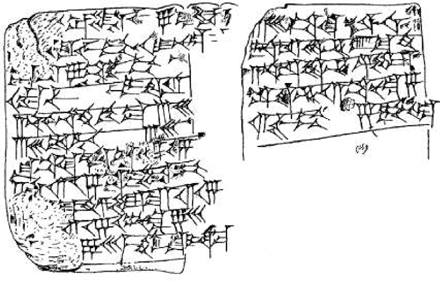
\includegraphics{images/ybc6967}}

הלוח תורגם לראשונה בידי אוטו נויגבאואר ואברהם זקס בספרם שעסק ספציפית
בטקסים מתמטיים בבליים - אותו ספר שבו צץ גם פלימפטון {\beginL 322\endL}
המפורסם יותר )ובפוסט עליו הרחבתי על נויגבאואר וזקס(.

מה כתוב בלוח? אני כמובן לא יודע לקרוא את זה ולכן מסתמך על תרגום קיים
שאביא פה ואחר כך אסביר מה הולך בו. כמה נקודות שכדאי לציין כבר עכשיו:
ראשית, המספרים כתובים פה בשיטה הבבלית, של ספירה על בסיס {\beginL 60\endL}.
זה אומר שכשכתוב \textquotedblright{\beginL 1,0\endL}\textquotedblleft{}
הכוונה היא למספר {\beginL 60\endL} )פעם אחת {\beginL 60\endL} ועוד
אפס פעמים {\beginL 1\endL}(, כשכתוב {\beginL 30\endL};{\beginL 3\endL}
הכוונה ל-\L{$3.5$} )כי {\beginL 30\endL} הוא חצי מ-{\beginL 60\endL}(
וכן הלאה. אם השיטה הזו מבלבלת אתכם פשוט תתעלמו; אני אשתמש במספרים
\textquotedblright רגילים\textquotedblleft{} בהמשך. שנית, בתרגום מופיעים
הביטויים \L{igum} ו-\L{igibum} בתור המספרים שמנסים למצוא - מה שאצלנו
היו אורכי הצלעות של המלבן. \textbf{ייתכן} שפירוש המילים הללו הו \textquotedblright הצלע
הקצרה של המלבן\textquotedblleft{} ו\textquotedblleft הצלע הארוכה של
המלבן\textquotedblleft , אבל כנראה יש להן הקשר רחב יותר ומשמעויות
נוספות )במקומות אחרים תרגמו את זה בתור \textquotedblright הופכיים\textquotedblleft{}
- כלומר, אלו שני מספרים שהופכיים זה לזה במובן זה שהכפולה שלהם היא
חזקה של {\beginL 60\endL}(. כמו כן בסוגריים מרובעים מופיע טקסט שלא
השתמר בלוח וזה הניחוש לגבי מה השחזור שלו אמור להיות. לבסוף, צריך לזכור
שאצל הבבלים לא היו מספרים שליליים, ולכן כשהם מוציאים שורש למספר, מבחינתם
יש לו רק שורש יחיד - החיובי.
\selectlanguage{english}%
\begin{quote}
{[}The igib{]}um exceeded the igum by 7. 

What are {[}the igum and{]} the igibum? 

As for you---halve 7, by which the igibum exceeded the igum, and
(the result is) 3;30. 

Multiply together 3;30 with 3;30, and (the result is) 12;15. 

To 12;15, which resulted for you, 

add {[}1,0, the produ{]}ct, and (the result is) 1,12;15. 

What is {[}the square root of 1{]},12;15?

(Answer:) 8;30. Lay down {[}8;30 and{]} 8;30, its equal, and then 

Subtract 3;30, the item, from the one, 

add (it) to the other. 

One is 12, the other 5. 

12 is the igibum, 5 the igum.
\end{quote}
\selectlanguage{hebrew}%
מה שיש לנו כאן הוא לימוד של שיטה כללית באמצעות פתרון של תרגיל ספציפי.
ה-\L{igum}, יהיה אשר יהיה פירוש המילה הזו, הוא ה-\L{$x$} שאנחנו מחפשים;
השורה הראשונה אומרת שה-\L{igibum} הוא \L{$x+7$}. השורה השניה מבקשת
מאיתנו למצוא אותם - זו הגדרת התרגיל. מהשורה השלישית כבר מגיע הפתרון
עצמו; בואו נכתוב אותו בלשון מודרנית. כזכור, בתרגיל הזה \L{$b=7$}
ו-\L{$c=-60$}, אז אני אכתוב בסוגריים גם את התיאור-באמצעות-סימבולים
של הדבר הקונקרטי שהלוח הבבלי עושה:
\begin{enumerate}
\item )שורה שלישית( מחלקים את {\beginL 7\endL} ב-\L{$2$} לקבלת \L{$3.5$}
)\L{$\frac{b}{2}$}( 
\item )שורה רביעית( מעלים את \L{$3.5$} בריבוע לקבלת {\beginL 12.25\endL}
)\L{$\frac{b^{2}}{4}$}(
\item )שורות חמישית ושישית( לתוצאה {\beginL 12.25\endL} מחברים את {\beginL 60\endL}
)\L{$\frac{b^{2}}{4}-c$}( ומקבלים \L{$72.25$}.
\item )שורות שביעית ושמינית( עכשיו מוציאים שורש ל-{\beginL 72.25\endL} )בלי
הסבר איך( ומקבלים {\beginL 8.5\endL} )\L{$\sqrt{\frac{b^{2}}{4}-c}$}(
\item )שורות תשיעית ועשירית( מחסרים מהתוצאה הזו את \L{$3.5$} שחישבנו קודם
ומקבלים {\beginL 5\endL} )\L{$\sqrt{\frac{b^{2}}{4}-c}-\frac{b}{2}$}(
\item )שורות אחד-עשר ושנים-עשר( מציגים את התוצאה: {\beginL 5\endL} ו-{\beginL 12\endL}.
\end{enumerate}
מה הולך פה? השלבים תואמים \textbf{במדויק} את החישוב של... של... של
מה בעצם? של שיטת ההשלמה לריבוע, או של שיטת המרחק מהממוצע? התשובה היא,
כמובן, שאת שניהם. \textbf{מבחינה מתמטית כל השיטות הללו זהות}. הטקסט
הבבלי לא נותן לנו רמזים לגבי \textbf{איך} הגיעו לעשות את החישובים
הללו - הוא מציג רק את האלגוריתם עצמו, בלי ה\textquotedblleft הערות
בקוד\textquotedblleft . מה שאפשר לעשות הוא רק להעלות השערות ולבסס
אותן על דברים אחרים שידועים על הבבלים והמתמטיקה הבבלית ולא נמצאים
בתוך הלוח הזה עצמו. ההיסטוריון של המתמטיקה \L{Jens Høyrup} הציע פרשות
אחת כזו שהיא נחמדה מאוד והצגתי אותה כבר פעמיים בבלוג - בפוסט על המשוואה
הריבועית ובפוסט על פלימפטון {\beginL 322\endL}, אבל למה לא פעם שלישית.
הנה התמונה שבה השתמשתי בעבר:

\L{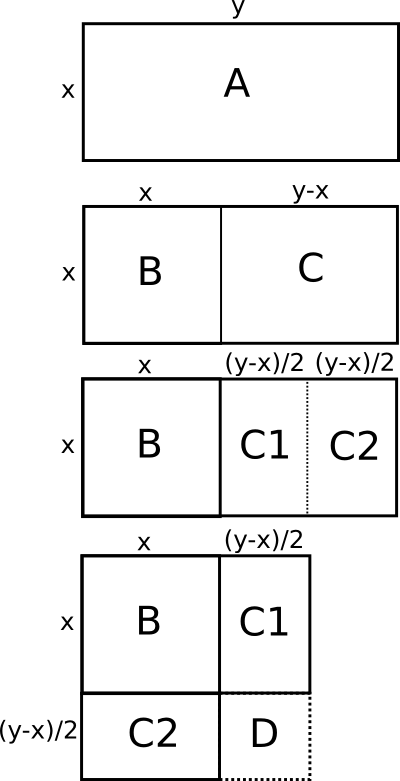
\includegraphics{images/completion_to_square}}

מה הולך פה? באיור הזה סימנתי את המלבן המדובר, ששטחו {\beginL 60\endL},
בתור \L{$A$}. את אורכי הצלעות סימנתי ב-\L{$x,y$}. זה אומר ש-\L{$y-x$}
הוא ה-\L{$b$} שלנו: ההפרש בין אורכי הצלעות. עכשיו, הרעיון הוא שהשיטה
עובדת כך: את \L{$A$} חותכים לשני חלקים - אחד הוא ריבוע שאורך צלעו
\L{$x$} ומסומן \L{$B$}, והשני הוא מלבן שמסומן \L{$C$} שאורך צלעו
האחת הוא \L{$x$} ואורך צלעו השניה הוא \textquotedblright מה שנשאר\textquotedblleft{}
אחרי שחתכנו מהצלע הארוכה חתיכה באורך \L{$x$} - כלומר, נשאר \L{$b$}.
סכום השטחים של שני המרובעים הללו הוא עדיין {\beginL 60\endL}.

עכשיו מגיע הטריק: לוקחים את \L{$C$} וחוצים אותו לשני חצאים, ואת אחד
מהחצאים מדביקים על החלק התחתון של \L{$B$}. קיבלנו שהוא משהו שהוא
\textquotedblright כמעט ריבוע\textquotedblleft{} חדש, וכדי לקבל ריבוע
אנחנו \textbf{משלימים אותו לריבוע} על ידי הוספת ריבוע קטן יותר, \L{$D$}.

אם זו אכן הטכניקה שהבבלים נקטו בה )ואין לדעת( אז שיטת הפתרון באמת
צצה מאליה באופן טבעי לגמרי. לוקחים את ההפרש, \L{$b=7$} ומחלקים אותו
ב-{\beginL 2\endL} - זה בדיוק שלב הפירוק של \L{$C$} לשני החלקים שלה.
עכשיו מחשבים את השטח של \L{$D$}, שהוא מה שנוסיף לצורה שלנו כדי להשלים
אותה לריבוע - השטח הזה הוא בדיוק \L{$\frac{b}{2}$} בריבוע, כי אורך
צלעו הוא \L{$\frac{b}{2}$}. עכשיו מוסיפים לשטח של \L{$D$} את השטח
של \L{$A$} המקורי - כלומר {\beginL 60\endL}, והתוצאה היא השטח של
הריבוע \textquotedblright הגדול\textquotedblleft . עכשיו מוציאים שורש
כדי לגלות את אורך צלע הריבוע הגדול - ומכיוון שאורך הצלע הזו הוא בדיוק
\L{$x+\frac{b}{2}$}, נשאר לחסר \L{$\frac{b}{2}$} מהתוצאה וסיימנו. 

אני לא יודע אם הבבלים אכן חשבו על זה בצורה הזו, אבל אני יודע ש\textbf{בסטנדרטים
של היום} התיאור הזה הוא יפהפה ואינטואיטיבי ולי הוא בהחלט עזר להפיל
אסימון לגבי שיטת ההשלמה לריבוע - עכשיו אנחנו רואים \textbf{בדיוק}
למה להוסיף \L{$\left(\frac{b}{2}\right)^{2}$} ורואים בעיניים איך
זה \textquotedblright משלים לריבוע\textquotedblleft{} משהו. אני בהחלט
חושב שזה משהו שיכול להיות נחמד מאוד אם יופיע בכל ספרי הלימוד, ולא
רק ההסבר \textquotedblright האלגברי\textquotedblleft .

ואיך ההסבר הגאומטרי הזה משתלב עם שיטת \textquotedblright המרחק מהממוצע\textquotedblleft ?
ובכן, נתחיל מכך שבשיטת \textquotedblright המרחק מהממוצע\textquotedblleft{}
אנחנו מסתכלים כאן על המקרה שבו הממוצע \textbf{שלילי}, כי \L{$b$}
אצלנו חיובי והממוצע הוא \L{$-\frac{b}{2}$}. הבבלים, כזכור, לא מתעניינים
בפתרון השלילי בכלל אלא רק בחיובי, אבל זה לא אומר שהפתרון השלילי לא
נוכח בתמונה: סימנתי בתור \L{$y$} את אורך הצלע הארוכה יותר; לא קשה
להשתכנע שבמקרה הזה \L{$-y$} הוא הפתרון השלילי של המשוואה \L{$x^{2}+bx+c$}
)כי \L{$x\cdot y=-c=60$} במקרה שלנו ו-\L{$b=y-x$} ולכן \L{$-b=x+\left(-y\right)$}(.
אז \textquotedblright הממוצע של הפתרונות\textquotedblleft{} הוא במקרה
הזה מינוס אורך הצלעות של ה-\L{$C$}-ים אחרי הפיצול, ומה שקראנו לו
\L{$z$} - \textquotedblright המרחק מהממוצע\textquotedblleft{} הוא
במקרה הנוכחי אורך צלע הריבוע הגדול שצריך להוסיף לממוצע כדי לקבל את
\L{$x$}. האינטואיציה של שיטת ממוצע הפתרונות נשמרת, לטעמי, בפתרון
הגאומטרי - \textquotedblright שוברים\textquotedblleft{} את המלבן \L{$y-x$}
לשני חלקים שווי גודל; אם לוקחים את התוצאה ומחסירים ממנה את החלק שעוד
מחובר אליה מקבלים את הצלע הקטנה יותר, ואם מוסיפים לה את מה שהסרנו
ממנה מקבלים את אורך הצלע השניה.

האם זה אומר שהבבלים \textquotedblright ידעו\textquotedblleft{} את השיטה
הזו? אני מקווה שבשלב הזה ברור למה השאלה הזו היא קצת חסרת משמעות. הבבלים
לא ניסו לפתור משוואה ממעלה שניה; הם ניסו לפתור בעיה של מציאת צלעות
של מלבן. מושג כמו \textquotedblright משוואה ממעלה שניה\textquotedblleft{}
היה זר להם; מושג כמו פתרונות שליליים של משוואה ממעלה שניה היה זר להם.
לקח למתמטיקה זמן להתחיל להסתכל על השאלות הללו כך ולנסות לפתור אותן
- וזה אנכרוניזם לנסות לחשוב על כך בצורה אחרת, ובטח שזה אנכרוניזם לומר
ש-{\beginL 4,000\endL} שנה אף אחד לא שם לב למשהו שנמצא מתחת לאף.

מצד שני, הטכניקות שעליהן מדובר פה? אנחנו רואים כאן היטב שהבבלים שלטו
בהן, וקרוב לודאי שהייתה להם אינטואיציה טובה לגביהן בדיוק כמונו. את
\textbf{האלגוריתם החישובי} שהשיטות האלגבריות שלנו מציעות הם בוודאי
ידעו בצורה מדויקת לגמרי. כל מה שנשאר הוא ה\textquotedblleft הערות
בקוד\textquotedblleft{} - וכאן הבבלים עוזרים לנו עם הגישה הגאומטרית
בדיוק כפי שאנחנו אולי היינו יכולים לעזור להם עם הגישה האלגברית. ככה
זה: מרבה שיטות, מרבה אינטואיציות, מרבה שמחה.
\end{document}
